\chapter{前置知识}
\label{chap:knowledge}

\section{Rust:依赖语言的程序设计}

\section{操作系统}

\subsection{Riscv}

\subsubsection{Sv39\pagescite{xv60}}

\textbf{地址格式与组成}

\begin{figure}[htb]
    \figureCapSet
    \centering
    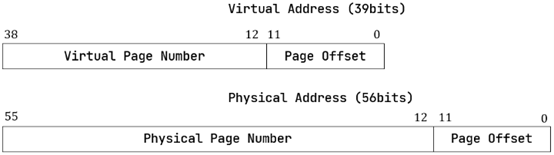
\includegraphics[width=.8\linewidth]{figure/c2/addressstructure.png}
    \caption{Sv39的地址格式}
    \label{figure:c2addressstructure}
\end{figure}

采用分页管理,单个页面的大小设置为 4KiB ,每个虚拟页面和物理页帧都对齐到这个页面大小,也就是说虚拟/物理地址区间 [0,4KiB) 为第 0 个虚拟页面/物理页帧,而 [4KiB,8KiB) 为第 1 个,以此类推。 4KiB 需要用 12 位字节地址来表示,因此虚拟地址和物理地址都被分成两部分:它们的低 12 位,即 [11:0] 被称为 页内偏移 (Page Offset) ,它描述一个地址指向的字节在它所在页面中的相对位置。而虚拟地址的高 27 位,即 [38:12] 为它的虚拟页号 VPN,同理物理地址的高 44 位,即 [55:12] 为它的物理页号 PPN,页号可以用来定位一个虚拟/物理地址属于哪一个虚拟页面/物理页帧。

地址转换是以页为单位进行的,在地址转换的前后地址的页内偏移部分不变。可以认为 MMU 只是从虚拟地址中取出 27 位虚拟页号,在页表中查到其对应的物理页号(如果存在的话),最后将得到的44位的物理页号与虚拟地址的12位页内偏移依序拼接到一起就变成了56位的物理地址。


\textbf{地址转换过程}

\begin{figure}[htb]
    \figureCapSet
    \centering
    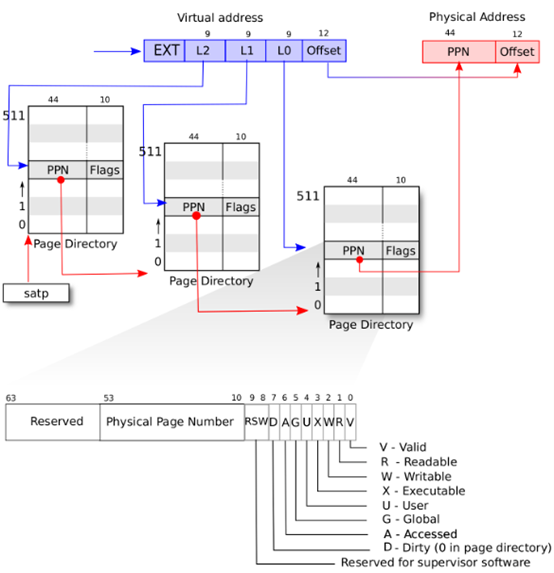
\includegraphics[width=.8\linewidth]{figure/c2/addressv2p.png}
    \caption{Sv39地址转换过程}
    \label{figure:c2addressv2p}
\end{figure}

在 SV39 模式中,采用三级页表,即将 27 位的虚拟页号分为三个等长的部分,第 26-18 位为一级页索引 VPN0 ,第 17-9 位为二级页索引 VPN1 ,第 8-0 位为三级页索引 VPN2 。

页表分为一级页表(多级页表的根节点),二级页表,三级页表(多级页表的叶节点)。每个页表都用 9 位索引,因此有 $2^9=512$ 个页表项,而每个页表项都是 8 字节,因此每个页表大小都为 $512\times 8=4 \mathrm{KiB}$ 。正好是一个物理页的大小。从而可以把一个页表放到一个物理页中,并用一个物理页号来描述它。事实上,一级页表的每个页表项中的物理页号可描述一个二级页表;二级页表的每个页表项中的物理页号可描述一个三级页表;三级页表中的页表项内容则和先前提到的页表项一样,包含物理页号,即描述一个要映射到的物理页。

具体来说,假设有虚拟地址$(VPN_{0} ,VPN_{1},VPN_{2},offset)$:
	首先会记录装载「当前所用的一级页表的物理页」的页号到 satp 寄存器中;
    \begin{itemize}
	\item 把 $VPN_{0}$ 作为偏移在一级页表的物理页中找到二级页表的物理页号;
	\item 把 $VPN_{1}$ 作为偏移在二级页表的物理页中找到三级页表的物理页号;
	\item 把 $VPN_{2}$ 作为偏移在三级页表的物理页中找到要访问位置的物理页号;
    \end{itemize}

	物理页号对应的物理页基址(即物理页号左移12位)加上 offset 就是虚拟地址对应的物理地址。

这样处理器通过这种多次转换,终于从虚拟页号找到了一级页表项,从而得出了物理页号和虚拟地址所对应的物理地址。刚才我们提到若页表项满足 R,W,X 都为 0,表明这个页表项指向下一级页表。在这里三级和二级页表项的 R,W,X 为 0 应该成立,因为它们指向了下一级页表。


\subsection{API与ABI}

从使用操作系统的角度会比较容易对操作系统内核的功能产生初步的认识。操作系统内核是一个提供各种服务的软件,其服务对象是应用程序,而用户是通过应用程序的服务间接获得操作系统的服务的,因此操作系统内核在一般用户面前是一个透明地。但应用程序需要访问操作系统获得操作系统的服务,这就需要通过操作系统的接口才能完成。操作系统与运行在用户态软件之间的接口形式就是应用程序二进制接口 (ABI, Application Binary Interface)。

操作系统不能只提供面向单一编程语言的函数库的编程接口 (API, Application Programming Interface) ,它的接口需要考虑对基于各种编程语言的应用支持,以及访问安全等因素,使得应用软件不能像访问函数库一样的直接访问操作系统内部函数,更不能直接读写操作系统内部的地址空间。为此,操作系统设计了一套安全可靠的二进制接口,即系统调用接口 (System Call Interface)。系统调用接口通常面向应用程序提供了 API 的描述,但在具体实现上,还需要提供 ABI 的接口描述规范。

在现代处理器的安全支持(特权级隔离,内存空间隔离等)下,应用程序就不能直接以函数调用的方式访问操作系统的函数,和直接读写操作系统的数据变量。不同类型的应用程序可以通过符合操作系统规定的系统调用接口,发出系统调用请求,来获得操作系统的服务。操作系统提供完服务后,返回应用程序继续执行。

\subsubsection{API 与 ABI 的区别}

应用程序二进制接口ABI是不同二进制代码片段的连接纽带。ABI定义了二进制机器代码级别的规则,主要包括基本数据类型、通用寄存器的使用、参数的传递规则、以及堆栈的使用等等。ABI与处理器和内存地址等硬件架构相关,是用来约束链接器 (Linker) 和汇编器 (Assembler) 的。在同一处理器下,基于不同高级语言编写的应用程序、库和操作系统,如果遵循同样的ABI定义,那么它们就能正确链接和执行。

应用程序编程接口API是不同源代码片段的连接纽带。API定义了一个源码级(如C语言)函数的参数,参数的类型,函数的返回值等。因此API是用来约束编译器 (Compiler) 的:一个API是给编译器的一些指令,它规定了源代码可以做以及不可以做哪些事。API与编程语言相关,如libc是基于C语言编写的标准库,那么基于C的应用程序就可以通过编译器建立与libc的联系,并能在运行中正确访问libc中的函数。


\section{异步}

\begin{lstlisting}[ caption = BREAKFIRST ]
enum FoodState {
    Cooked,
    Eating,
    Finished,
};
async fn milk () { /* ... */ }
async fn bread () { /* ... */ }
async fn eat () {
    /* ... */
    milk.await;
    bread.await;
    /* ... */
}

\end{lstlisting}


